\documentclass[10pt,]{book}
\usepackage{lmodern}
\usepackage{amssymb,amsmath}
\usepackage{ifxetex,ifluatex}
\usepackage{fixltx2e} % provides \textsubscript
\ifnum 0\ifxetex 1\fi\ifluatex 1\fi=0 % if pdftex
  \usepackage[T1]{fontenc}
  \usepackage[utf8]{inputenc}
\else % if luatex or xelatex
  \ifxetex
    \usepackage{mathspec}
  \else
    \usepackage{fontspec}
  \fi
  \defaultfontfeatures{Ligatures=TeX,Scale=MatchLowercase}
\fi
% use upquote if available, for straight quotes in verbatim environments
\IfFileExists{upquote.sty}{\usepackage{upquote}}{}
% use microtype if available
\IfFileExists{microtype.sty}{%
\usepackage{microtype}
\UseMicrotypeSet[protrusion]{basicmath} % disable protrusion for tt fonts
}{}
\usepackage[margin=1in]{geometry}
\usepackage{hyperref}
\PassOptionsToPackage{usenames,dvipsnames}{color} % color is loaded by hyperref
\hypersetup{unicode=true,
            pdftitle={Gráficos con R},
            colorlinks=true,
            linkcolor=Maroon,
            citecolor=Blue,
            urlcolor=Blue,
            breaklinks=true}
\urlstyle{same}  % don't use monospace font for urls
\usepackage{natbib}
\bibliographystyle{apalike}
\usepackage{color}
\usepackage{fancyvrb}
\newcommand{\VerbBar}{|}
\newcommand{\VERB}{\Verb[commandchars=\\\{\}]}
\DefineVerbatimEnvironment{Highlighting}{Verbatim}{commandchars=\\\{\}}
% Add ',fontsize=\small' for more characters per line
\usepackage{framed}
\definecolor{shadecolor}{RGB}{248,248,248}
\newenvironment{Shaded}{\begin{snugshade}}{\end{snugshade}}
\newcommand{\KeywordTok}[1]{\textcolor[rgb]{0.13,0.29,0.53}{\textbf{{#1}}}}
\newcommand{\DataTypeTok}[1]{\textcolor[rgb]{0.13,0.29,0.53}{{#1}}}
\newcommand{\DecValTok}[1]{\textcolor[rgb]{0.00,0.00,0.81}{{#1}}}
\newcommand{\BaseNTok}[1]{\textcolor[rgb]{0.00,0.00,0.81}{{#1}}}
\newcommand{\FloatTok}[1]{\textcolor[rgb]{0.00,0.00,0.81}{{#1}}}
\newcommand{\ConstantTok}[1]{\textcolor[rgb]{0.00,0.00,0.00}{{#1}}}
\newcommand{\CharTok}[1]{\textcolor[rgb]{0.31,0.60,0.02}{{#1}}}
\newcommand{\SpecialCharTok}[1]{\textcolor[rgb]{0.00,0.00,0.00}{{#1}}}
\newcommand{\StringTok}[1]{\textcolor[rgb]{0.31,0.60,0.02}{{#1}}}
\newcommand{\VerbatimStringTok}[1]{\textcolor[rgb]{0.31,0.60,0.02}{{#1}}}
\newcommand{\SpecialStringTok}[1]{\textcolor[rgb]{0.31,0.60,0.02}{{#1}}}
\newcommand{\ImportTok}[1]{{#1}}
\newcommand{\CommentTok}[1]{\textcolor[rgb]{0.56,0.35,0.01}{\textit{{#1}}}}
\newcommand{\DocumentationTok}[1]{\textcolor[rgb]{0.56,0.35,0.01}{\textbf{\textit{{#1}}}}}
\newcommand{\AnnotationTok}[1]{\textcolor[rgb]{0.56,0.35,0.01}{\textbf{\textit{{#1}}}}}
\newcommand{\CommentVarTok}[1]{\textcolor[rgb]{0.56,0.35,0.01}{\textbf{\textit{{#1}}}}}
\newcommand{\OtherTok}[1]{\textcolor[rgb]{0.56,0.35,0.01}{{#1}}}
\newcommand{\FunctionTok}[1]{\textcolor[rgb]{0.00,0.00,0.00}{{#1}}}
\newcommand{\VariableTok}[1]{\textcolor[rgb]{0.00,0.00,0.00}{{#1}}}
\newcommand{\ControlFlowTok}[1]{\textcolor[rgb]{0.13,0.29,0.53}{\textbf{{#1}}}}
\newcommand{\OperatorTok}[1]{\textcolor[rgb]{0.81,0.36,0.00}{\textbf{{#1}}}}
\newcommand{\BuiltInTok}[1]{{#1}}
\newcommand{\ExtensionTok}[1]{{#1}}
\newcommand{\PreprocessorTok}[1]{\textcolor[rgb]{0.56,0.35,0.01}{\textit{{#1}}}}
\newcommand{\AttributeTok}[1]{\textcolor[rgb]{0.77,0.63,0.00}{{#1}}}
\newcommand{\RegionMarkerTok}[1]{{#1}}
\newcommand{\InformationTok}[1]{\textcolor[rgb]{0.56,0.35,0.01}{\textbf{\textit{{#1}}}}}
\newcommand{\WarningTok}[1]{\textcolor[rgb]{0.56,0.35,0.01}{\textbf{\textit{{#1}}}}}
\newcommand{\AlertTok}[1]{\textcolor[rgb]{0.94,0.16,0.16}{{#1}}}
\newcommand{\ErrorTok}[1]{\textcolor[rgb]{0.64,0.00,0.00}{\textbf{{#1}}}}
\newcommand{\NormalTok}[1]{{#1}}
\usepackage{longtable,booktabs}
\usepackage{graphicx,grffile}
\makeatletter
\def\maxwidth{\ifdim\Gin@nat@width>\linewidth\linewidth\else\Gin@nat@width\fi}
\def\maxheight{\ifdim\Gin@nat@height>\textheight\textheight\else\Gin@nat@height\fi}
\makeatother
% Scale images if necessary, so that they will not overflow the page
% margins by default, and it is still possible to overwrite the defaults
% using explicit options in \includegraphics[width, height, ...]{}
\setkeys{Gin}{width=\maxwidth,height=\maxheight,keepaspectratio}
\IfFileExists{parskip.sty}{%
\usepackage{parskip}
}{% else
\setlength{\parindent}{0pt}
\setlength{\parskip}{6pt plus 2pt minus 1pt}
}
\setlength{\emergencystretch}{3em}  % prevent overfull lines
\providecommand{\tightlist}{%
  \setlength{\itemsep}{0pt}\setlength{\parskip}{0pt}}
\setcounter{secnumdepth}{5}
% Redefines (sub)paragraphs to behave more like sections
\ifx\paragraph\undefined\else
\let\oldparagraph\paragraph
\renewcommand{\paragraph}[1]{\oldparagraph{#1}\mbox{}}
\fi
\ifx\subparagraph\undefined\else
\let\oldsubparagraph\subparagraph
\renewcommand{\subparagraph}[1]{\oldsubparagraph{#1}\mbox{}}
\fi

%%% Use protect on footnotes to avoid problems with footnotes in titles
\let\rmarkdownfootnote\footnote%
\def\footnote{\protect\rmarkdownfootnote}

%%% Change title format to be more compact
\usepackage{titling}

% Create subtitle command for use in maketitle
\newcommand{\subtitle}[1]{
  \posttitle{
    \begin{center}\large#1\end{center}
    }
}

\setlength{\droptitle}{-2em}
  \title{Gráficos con R}
  \pretitle{\vspace{\droptitle}\centering\huge}
  \posttitle{\par}
  \author{Juan Carlos Correa Morales\\
Freddy Hernández Barajas}
  \preauthor{\centering\large\emph}
  \postauthor{\par}
  \predate{\centering\large\emph}
  \postdate{\par}
  \date{2016-12-04}

\usepackage{booktabs}
\usepackage[spanish]{babel}
\decimalpoint
\selectlanguage{spanish}

% Comandos para escribir nombres de paquetes, programas y codigos
\newcommand{\pkg}[1]{{\normalfont\fontseries{b}\selectfont #1}}
\let\proglang=\textsf
\let\code=\texttt

% Para crear el indice
\usepackage{makeidx}
\makeindex

\begin{document}
\maketitle

{
\hypersetup{linkcolor=black}
\setcounter{tocdepth}{1}
\tableofcontents
}
\listoftables
\listoffigures
\chapter*{Prefacio}\label{prefacio}
\addcontentsline{toc}{chapter}{Prefacio}

Este libro \ldots{}

\chapter{Introducción}\label{introduccion}

\section{Orígenes} \label{sec:origenes}

\proglang{R} es un lenguaje de programación usado para realizar
procedimientos estadísticos y gráficos de alto nivel, este lenguaje fue
creado en 1993 por los profesores e investigadores Robert Gentleman y
Ross Ihaka. Inicialmente el lenguaje se usó para apoyar los cursos que
tenían a su cargo los profesores, pero luego de ver la utilidad de la
herramienta desarrollada, decidieron colocar copias de \proglang{R} en
StatLib. A partir de 1995 el código fuente de \proglang{R} está
disponible bajo licencia GNU GPL para sistemas operativos Windows,
Macintosh y distribuciones Unix/Linux. La comunidad de usuarios de
\proglang{R} en el mundo es muy grande y los usuarios cuentan con
diferentes espacios para interactuar, a continuación una lista no
exhaustiva de los sitios más populares relacionados con \proglang{R}:

\begin{itemize}
\tightlist
\item
  \href{https://www.r-bloggers.com/}{Rbloggers}.
\item
  \href{http://r-es.org/}{Comunidad hispana de \proglang{R}}.
\item
  \href{http://r.789695.n4.nabble.com/}{Nabble}.
\item
  \href{http://r-br.2285057.n4.nabble.com/}{Foro en portugués}.
\item
  \href{http://stackoverflow.com/questions/tagged/r}{Stackoverflow}.
\item
  \href{http://stats.stackexchange.com/questions/tagged/r}{Cross
  Validated}.
\item
  \href{https://stat.ethz.ch/mailman/listinfo/r-help}{\proglang{R}-Help
  Mailing List}.
\item
  \href{http://blog.revolutionanalytics.com/}{Revolutions}.
\item
  \href{https://www.r-statistics.com/}{\proglang{R}-statistics blog}.
\item
  \href{https://rdatamining.wordpress.com/}{RDataMining}.
\end{itemize}

\begin{figure}

{\centering 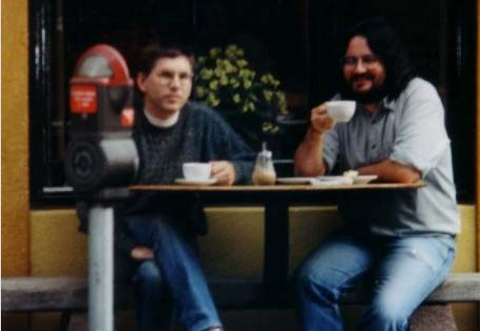
\includegraphics[width=2.4in]{images/Robert_Roos} 

}

\caption{Robert Gentleman (izquierda) y Ross Ihaka (derecha) creadores de R.}\label{fig:unnamed-chunk-1}
\end{figure}

\section{Descarga e instalación} \label{sec:descarga}

Para realizar la instalación de \proglang{R} usted debe visitar la
página del CRAN (\textit{Comprehensive R Archive Network}) disponible en
este \href{https://cran.r-project.org/}{enlace}. Una vez ingrese a la
página encontrará un cuadro similar al mostrado en la Figura
\ref{fig:cran} donde aparecen los enlaces de la instalación para los
sistemas operativos Linux, Mac y Windows.

\begin{figure}

{\centering 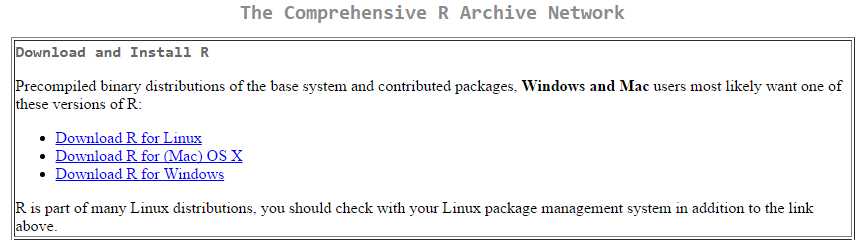
\includegraphics[width=4.54in]{images/cran} 

}

\caption{Página del Cran.}\label{fig:cran}
\end{figure}

Supongamos que se desea instalar \proglang{R} en Windows, para esto se
debe dar clic sobre el hiperenlace
\textcolor{BurntOrange}{Download R for Windows} de la Figura
\ref{fig:cran}. Una vez hecho esto se abrirá una página con el contenido
mostrado en la Figura \ref{fig:inst1}. Una vez ingrese a esa nueva
página usted debe dar clic sobre el hiperenlace
\textcolor{BurntOrange}{install R for the first time} como es señalado
por la flecha roja en la Figura \ref{fig:inst1}.

\begin{figure}

{\centering 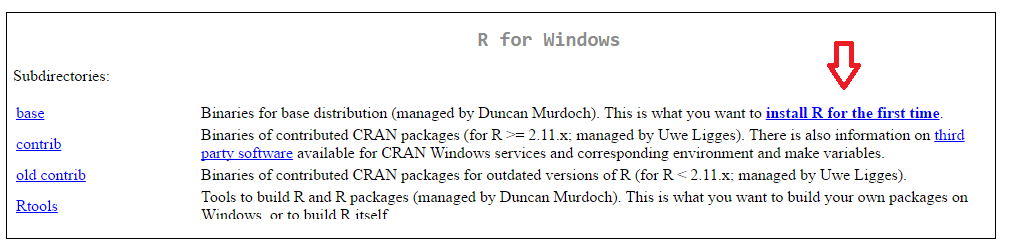
\includegraphics[width=5.31in]{images/instalacion1} 

}

\caption{Página de instalación para la primera ocasión.}\label{fig:inst1}
\end{figure}

Luego de esto se abrirá otra página con un encabezado similar al
mostrado en la Figura \ref{fig:inst2}, al momento de capturar la figura
la versión actual de \proglang{R} era 3.2.5 pero seguramente en este
momento usted tendrá disponible una versión actualizada. Una vez allí
uste debe dar clic sobre
\textcolor{BurntOrange}{Download R 3.2.5 for Windows} como es señalado
por la flecha verde. Luego de esto se descargará el instalador
\proglang{R} en el computador el cual deberá ser instalado con las
opciones que vienen por defecto.

\begin{figure}

{\centering 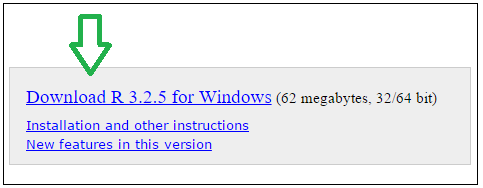
\includegraphics[width=2.54in]{images/instalacion2} 

}

\caption{Página de descarga.}\label{fig:inst2}
\end{figure}

Se recomienda observar el siguiente video didáctico de instalación de
\proglang{R} disponible en este
\href{http://tinyurl.com/jd7b9ks}{enlace} para facilitar la tarea de
instalación.

\section{Apariencia del programa} \label{sec:apariencia}

Una vez que esté instalado \proglang{R} en su computador, usted podrá
acceder a él por la lista de programas o por medio del acceso directo
que quedó en el escritorio, en la Figura \ref{fig:rlogo} se muestra la
apariencia del acceso directo para ingresar a \proglang{R}.

\begin{figure}

{\centering 
\includegraphics[width=1.14in]{images/rlogo} 

}

\caption{Apariencia del acceso directo para ingresar a R.}\label{fig:rlogo}
\end{figure}

Al abrir \proglang{R} aparecerá en la pantalla de su computador algo
similar a lo que está en la Figura \ref{fig:pantalla}. La ventana
izquierda se llama consola y es donde se ingresan las instrucciones, una
vez que se construye un gráfico se activa otra ventana llamada ventana
gráfica. Cualquier usuario puede modificar la posición y tamaños de
estas ventanas, puede cambiar el tipo y tamaño de las letras en la
consola, para hacer esto se deben explorar las opciones de
\textit{editar} en la barra de herramientas.

\begin{figure}

{\centering 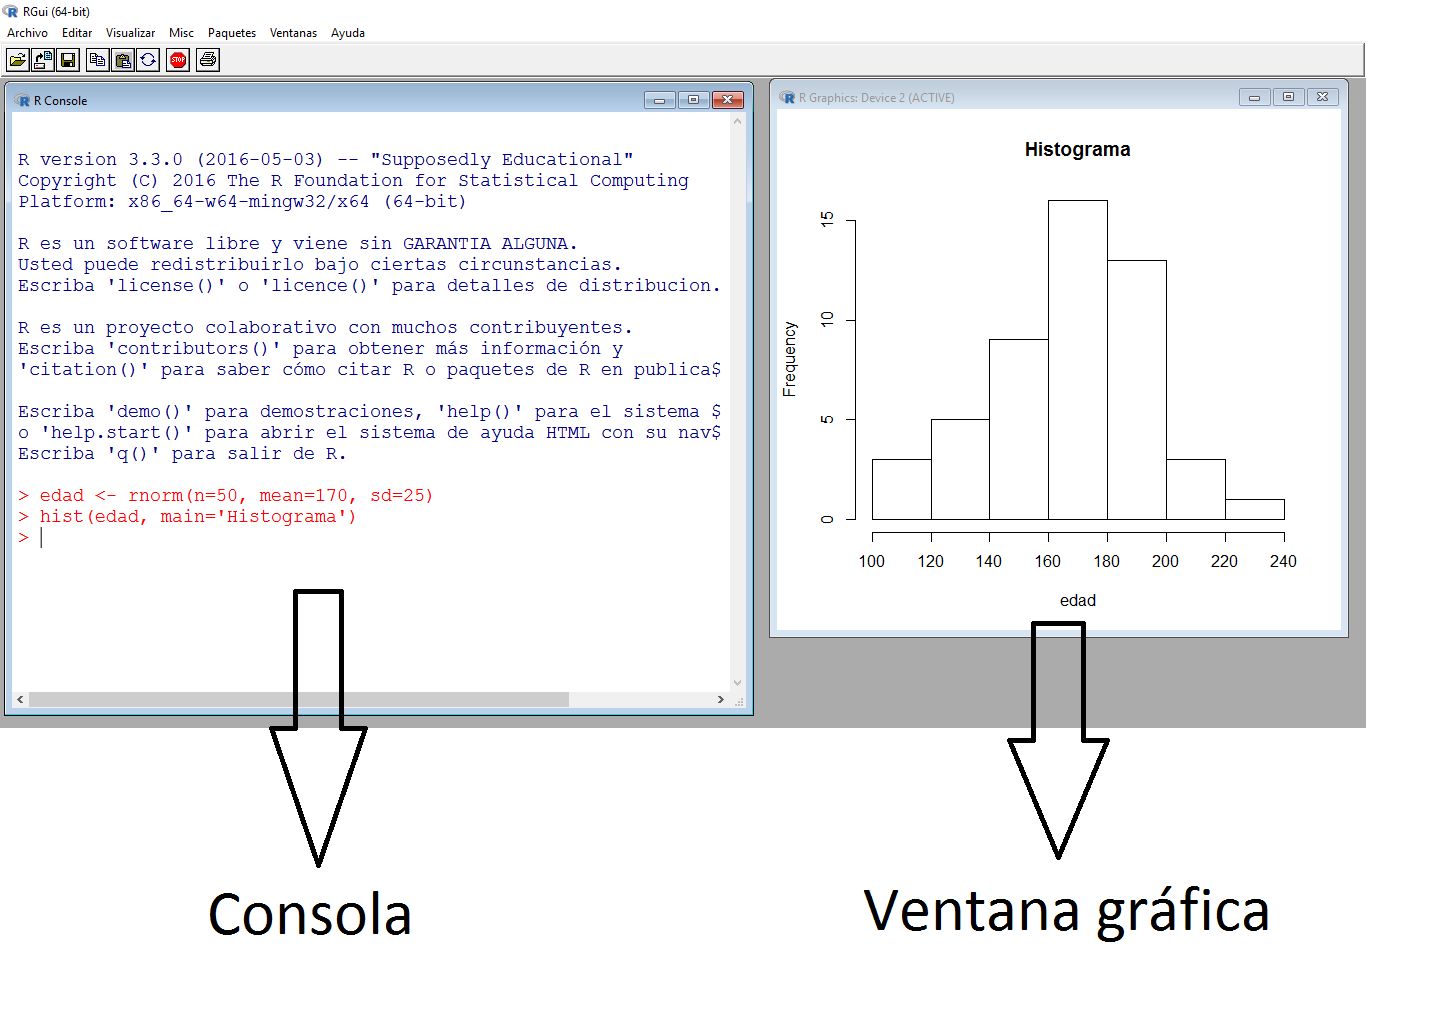
\includegraphics[width=3.6in]{images/Rpantallazo} 

}

\caption{Apariencia de R.}\label{fig:pantalla}
\end{figure}

\section{Tipos de objetos} \label{sec:objetos}

En \proglang{R} existen varios tipos de objectos \index{objetos} que
permiten que el usuario pueda almacenar la información para realizar
procedimientos estadísticos y gráficos. Los principales objetos en
\proglang{R} son vectores, matrices, arreglos, marcos de datos y listas.
A continuación se presentan las características de estos objetos y la
forma para crearlos.

\subsection{Vectores}

Los vectores \index{vectores} son arreglos ordenados en los cuales se
puede almacenar información de tipo numérico (variable cuantitativa),
alfanumérico (variable cualitativa) o lógico (\texttt{TRUE} o
\texttt{FALSE}), pero no mezclas de éstos. La función de \proglang{R}
para crear un vector es \texttt{c()} y que significa concatenar; dentro
de los paréntesis de esta función se ubica la información a almacenar.
Una vez construído el vector se acostumbra a etiquetarlo con un nombre
corto y representativo de la información que almacena, la asignación se
hace por medio del operador \texttt{\textless{}-} entre el nombre y el
vector.

A continuación se presenta un ejemplo de cómo crear tres vectores que
contienen las respuestas de cinco personas a tres preguntas que se les
realizaron.

\begin{Shaded}
\begin{Highlighting}[]
\NormalTok{edad <-}\StringTok{ }\KeywordTok{c}\NormalTok{(}\DecValTok{15}\NormalTok{, }\DecValTok{19}\NormalTok{, }\DecValTok{13}\NormalTok{, }\OtherTok{NA}\NormalTok{, }\DecValTok{20}\NormalTok{)}
\NormalTok{deporte <-}\StringTok{ }\KeywordTok{c}\NormalTok{(}\OtherTok{TRUE}\NormalTok{, }\OtherTok{TRUE}\NormalTok{, }\OtherTok{NA}\NormalTok{, }\OtherTok{FALSE}\NormalTok{, }\OtherTok{TRUE}\NormalTok{)}
\NormalTok{comic.fav <-}\StringTok{ }\KeywordTok{c}\NormalTok{(}\OtherTok{NA}\NormalTok{, }\StringTok{'Superman'}\NormalTok{, }\StringTok{'Batman'}\NormalTok{, }\OtherTok{NA}\NormalTok{, }\StringTok{'Batman'}\NormalTok{)}
\end{Highlighting}
\end{Shaded}

El vector \texttt{edad} es un vector cuantitativo y contiene las edades
de las 5 personas. En la cuarta posición del vector se colocó el símbolo
\texttt{NA} que significa \textit{Not Available} debido a que no se
registró la edad para esa persona. Al hacer una asignación se acostumbra
a dejar un espacio antes y después del operador \texttt{\textless{}-} de
asignación. El segundo vector es llamado \texttt{deporte} y es un vector
lógico que almacena las respuestas a la pregunta de si la persona
practica deporte, nuevamente aquí hay un \texttt{NA} para la tercera
persona. El último vector \texttt{comic.fav} contiene la información del
cómic favorito de cada persona, como esta variable es cualitativa es
necesario usar las comillas
\texttt{\textquotesingle{}\ \textquotesingle{}} para encerrar las
respuestas. Cuando se usa \texttt{NA} para representar una información
\textit{Not Available} NO SE DEBEN usar las comillas
\texttt{\textquotesingle{}\ \textquotesingle{}}.

Nota: es posible usar comillas sencillas
\texttt{\textquotesingle{}foo\textquotesingle{}} o comillas dobles
\texttt{"foo"} para ingresar valores de una variable cualitativa.

Si se desea ver lo que está almacenado en cada uno de estos vectores, se
debe escribir en la consola de \proglang{R} el nombre de uno de los
objetos y luego se presiona la tecla \textit{enter} o \textit{intro}, al
realizar esto lo que se obtiene se muestra a continuación.

\begin{Shaded}
\begin{Highlighting}[]
\NormalTok{edad}
\end{Highlighting}
\end{Shaded}

\begin{verbatim}
## [1] 15 19 13 NA 20
\end{verbatim}

\begin{Shaded}
\begin{Highlighting}[]
\NormalTok{deporte}
\end{Highlighting}
\end{Shaded}

\begin{verbatim}
## [1]  TRUE  TRUE    NA FALSE  TRUE
\end{verbatim}

\begin{Shaded}
\begin{Highlighting}[]
\NormalTok{comic.fav}
\end{Highlighting}
\end{Shaded}

\begin{verbatim}
## [1] NA         "Superman" "Batman"   NA         "Batman"
\end{verbatim}

\subsection{Matrices}

Las matrices \index{matrices} son arreglos rectangulares de filas y
columnas con información numérica, alfanumérica o lógica. Para construir
una matriz se usa la función \texttt{matrix(\ )}. Por ejemplo, para
crear una matriz de 4 filas y 5 columnas (de dimensión \(4 \times 5\))
con los primeros 20 números positivos se escribe el código siguiente en
la consola.

\begin{Shaded}
\begin{Highlighting}[]
\NormalTok{mimatriz <-}\StringTok{ }\KeywordTok{matrix}\NormalTok{(}\DataTypeTok{data=}\DecValTok{1}\NormalTok{:}\DecValTok{20}\NormalTok{, }\DataTypeTok{nrow=}\DecValTok{4}\NormalTok{, }\DataTypeTok{ncol=}\DecValTok{5}\NormalTok{, }\DataTypeTok{byrow=}\OtherTok{FALSE}\NormalTok{)}
\end{Highlighting}
\end{Shaded}

El argumento \texttt{data} de la función sirve para indicar los datos
que se van a almacenar en la matriz, los argumentos \texttt{nrow} y
\texttt{ncol} sirven para definir la dimensión de la matriz y por último
el argumento \texttt{byrow} sirve para indicar si la información
contenida en \texttt{data} se debe ingresar por filas o no. Para
observar lo que quedó almacenado en el objeto \texttt{mimatriz} se
escribe en la consola el nombre del objeto seguido de la tecla
\textit{enter} o \textit{intro}.

\begin{Shaded}
\begin{Highlighting}[]
\NormalTok{mimatriz}
\end{Highlighting}
\end{Shaded}

\begin{verbatim}
##      [,1] [,2] [,3] [,4] [,5]
## [1,]    1    5    9   13   17
## [2,]    2    6   10   14   18
## [3,]    3    7   11   15   19
## [4,]    4    8   12   16   20
\end{verbatim}

\subsection{Arreglos}

Un arreglo \index{arreglo} es una matriz de varias dimensiones con
información numérica, alfanumérica o lógica. Para construir una arreglo
se usa la función \texttt{array(\ )}. Por ejemplo, para crear un arreglo
de \(3 \times 4 \times 2\) con las primeras 24 letras minúsculas del
alfabeto se escribe el siguiente código.

\begin{Shaded}
\begin{Highlighting}[]
\NormalTok{miarray <-}\StringTok{ }\KeywordTok{array}\NormalTok{(}\DataTypeTok{data=}\NormalTok{letters[}\DecValTok{1}\NormalTok{:}\DecValTok{24}\NormalTok{], }\DataTypeTok{dim=}\KeywordTok{c}\NormalTok{(}\DecValTok{3}\NormalTok{, }\DecValTok{4}\NormalTok{, }\DecValTok{2}\NormalTok{))}
\end{Highlighting}
\end{Shaded}

El argumento \texttt{data} de la función sirve para indicar los datos
que se van a almacenar en el arreglo y el argumento \texttt{dim} sirve
para indicar las dimensiones del arreglo. Para observar lo que quedó
almacenado en el objeto \texttt{miarray} se escribe en la consola lo
siguiente.

\begin{Shaded}
\begin{Highlighting}[]
\NormalTok{miarray}
\end{Highlighting}
\end{Shaded}

\begin{verbatim}
## , , 1
## 
##      [,1] [,2] [,3] [,4]
## [1,] "a"  "d"  "g"  "j" 
## [2,] "b"  "e"  "h"  "k" 
## [3,] "c"  "f"  "i"  "l" 
## 
## , , 2
## 
##      [,1] [,2] [,3] [,4]
## [1,] "m"  "p"  "s"  "v" 
## [2,] "n"  "q"  "t"  "w" 
## [3,] "o"  "r"  "u"  "x"
\end{verbatim}

\subsection{Marco de datos}

El marco de datos \index{marco de datos} o \textit{data frame} es uno de
los objetos más utilizados porque permite agrupar vectores con
información de diferente tipo (numérica, alfanumérica o lógica) en un
mismo objeto, la única restricción es que los vectores deben tener la
misma longitud. Para crear un marco de datos se usa la función
\texttt{data.frame(\ )}, como ejemplo vamos a crear un marco de datos
con los vectores \texttt{edad}, \texttt{deporte} y \texttt{comic.fav}
definidos anteriormente.

\begin{Shaded}
\begin{Highlighting}[]
\NormalTok{mimarco <-}\StringTok{ }\KeywordTok{data.frame}\NormalTok{(edad, deporte, comic.fav)}
\end{Highlighting}
\end{Shaded}

Una vez creado el objeto \texttt{mimarco} podemos ver el objeto
escribiendo su nombre en la consola, a continuación se muestra lo que se
obtiene.

\begin{Shaded}
\begin{Highlighting}[]
\NormalTok{mimarco}
\end{Highlighting}
\end{Shaded}

\begin{verbatim}
##   edad deporte comic.fav
## 1   15    TRUE      <NA>
## 2   19    TRUE  Superman
## 3   13      NA    Batman
## 4   NA   FALSE      <NA>
## 5   20    TRUE    Batman
\end{verbatim}

De la salida anterior vemos que el marco de datos tiene 3 variables
(columnas) cuyos nombres coinciden con los nombres de los vectores
creados anteriormente, los números consecutivos al lado izquierdo son
sólo de referencia y permiten identificar la información para cada
persona en la base de datos.

\subsection{Listas}

Las listas \index{lista} son otro tipo de objeto muy usado para
almacenar objetos de diferente tipo. La instrucción para crear una lista
es \texttt{list(\ )}. A continuación vamos a crear una lista que
contiene tres objetos: un vector con 5 números aleatorios llamado
\texttt{mivector}, una matriz de dimensión \(6 \times 2\) con los
primeros doce números enteros positivos llamada \texttt{matriz2} y el
tercer objeto será el marco de datos \texttt{mimarco} creado en el
apartado anterior. Las instrucciones para crear la lista requerida se
muestran a continuación.

\begin{Shaded}
\begin{Highlighting}[]
\KeywordTok{set.seed}\NormalTok{(}\DecValTok{12345}\NormalTok{)}
\NormalTok{mivector <-}\StringTok{ }\KeywordTok{runif}\NormalTok{(}\DataTypeTok{n=}\DecValTok{5}\NormalTok{)}
\NormalTok{matriz2 <-}\StringTok{ }\KeywordTok{matrix}\NormalTok{(}\DataTypeTok{data=}\DecValTok{1}\NormalTok{:}\DecValTok{12}\NormalTok{, }\DataTypeTok{ncol=}\DecValTok{6}\NormalTok{)}
\NormalTok{milista <-}\StringTok{ }\KeywordTok{list}\NormalTok{(}\DataTypeTok{E1=}\NormalTok{mivector, }\DataTypeTok{E2=}\NormalTok{matriz2, }\DataTypeTok{E3=}\NormalTok{mimarco)}
\end{Highlighting}
\end{Shaded}

La función \texttt{set.seed} de la línea número 1 sirve para fijar la
semilla de tal manera que los números aleatorios generados en la segunda
línea con la función \texttt{runif} sean siempre los mismos. En la
última línea del código anterior se construye la lista, dentro de la
función \texttt{list} se colocan los tres objetos \texttt{mivector},
\texttt{matriz2} y \texttt{mimarco}. Es posible colocarle un nombre
especial a cada uno de los elementos de la lista, en este ejemplo se
colocaron los nombres \texttt{E1}, \texttt{E2} y \texttt{E3} para cada
uno de los tres elementos. Para observar lo que quedó almacenado en la
lista se escribe \texttt{milista} en la consola y el resultado se
muestra a continuación.

\begin{Shaded}
\begin{Highlighting}[]
\NormalTok{milista}
\end{Highlighting}
\end{Shaded}

\begin{verbatim}
## $E1
## [1] 0.7209039 0.8757732 0.7609823 0.8861246 0.4564810
## 
## $E2
##      [,1] [,2] [,3] [,4] [,5] [,6]
## [1,]    1    3    5    7    9   11
## [2,]    2    4    6    8   10   12
## 
## $E3
##   edad deporte comic.fav
## 1   15    TRUE      <NA>
## 2   19    TRUE  Superman
## 3   13      NA    Batman
## 4   NA   FALSE      <NA>
## 5   20    TRUE    Batman
\end{verbatim}

\section{Guía de estilo para la escritura en R} \label{sec:estilo}

Así como en el español existen reglas ortográficas, la escritura de
códigos en \proglang{R} también tiene unas reglas que se recomienda
seguir para evitar confusiones. Tener una buena guía de estilo
\index{guía de estilo} es importante para que el código creado por usted
sea fácilmente entendido por sus lectores \citep{rpackages}. No existe
una única y mejor guía de estilo para escritura en \proglang{R}, sin
embargo aquí vamos a mostrar unas sugerencias basadas en la guía llamada
\href{https://google.github.io/styleguide/Rguide.xml}{\textit{Google's R style guide}}.

\subsection{Nombres de los archivos}

Se sugiere que el nombre usado para nombrar un archivo tenga sentido y
que termine con extensión .R. A continuación dos ejemplos de como
nombrar mal y bien un archivo.

\begin{itemize}
    \item Mal: \verb|hola.R|
    \item Bien: \verb|analisis_icfes.R|
\end{itemize}

\subsection{Nombres de los objetos}

Se recomienda no usar los símbolos \texttt{\_} y \texttt{-} dentro de
los nombres de objetos. Para las variables es preferible usar letras
minúsculas y separar las palabras con puntos (\texttt{peso.maiz}) o
utilizar la notación camello iniciando en minúscula (\texttt{pesoMaiz}).
Para las funciones se recomienda usar la notación camello iniciando
todas la palabras en mayúscula (\texttt{PlotRes}). Para los nombres de
las constantes se recomienda que inicien con la letra k
(\texttt{kPrecioBus}). A continuación ejemplos de buenas y malas
prácticas.

Para variables:

\begin{itemize}
    \item Bien: \verb|avg.clicks|
    \item Aceptable: \verb|avgClicks|
    \item Mal: \verb|avg_Clicks|
\end{itemize}

Para funciones:

\begin{itemize}
    \item Bien: \verb|CalculateAvgClicks| 
    \item Mal: \verb|calculate_avg_clicks| , \verb|calculateAvgClicks|
\end{itemize}

\subsection{Longitud de una línea de código}

Se recomienda que cada línea tenga como máximo 80 caracteres. Si una
línea es muy larga se debe cortar siempre por una coma.

\subsection{Espacios}

Use espacios alrededor de todos los operadores binarios (=, +, -,
\textless{}-, etc.). Los espacios alrededor del símbolo ``='' son
opcionales cuando se usan para ingresar valores dentro de una función.
Así como en español, nunca coloque espacio antes de una coma, pero
siempre use espacio luego de una coma. A continuación ejemplos de buenas
y malas prácticas.

\begin{Shaded}
\begin{Highlighting}[]
\NormalTok{tab <-}\StringTok{ }\KeywordTok{table}\NormalTok{(df[df$days <}\StringTok{ }\DecValTok{0}\NormalTok{, }\DecValTok{2}\NormalTok{])  }\CommentTok{# Bien}
\NormalTok{tot <-}\StringTok{ }\KeywordTok{sum}\NormalTok{(x[, }\DecValTok{1}\NormalTok{])                }\CommentTok{# Bien}
\NormalTok{tot <-}\StringTok{ }\KeywordTok{sum}\NormalTok{(x[}\DecValTok{1}\NormalTok{, ])                }\CommentTok{# Bien}
\NormalTok{tab <-}\StringTok{ }\KeywordTok{table}\NormalTok{(df[df$days<}\DecValTok{0}\NormalTok{, }\DecValTok{2}\NormalTok{])    }\CommentTok{# Faltan espacios alrededor '<' }
\NormalTok{tab <-}\StringTok{ }\KeywordTok{table}\NormalTok{(df[df$days <}\StringTok{ }\DecValTok{0}\NormalTok{,}\DecValTok{2}\NormalTok{])   }\CommentTok{# Falta espacio luego de coma}
\NormalTok{tab <-}\StringTok{ }\KeywordTok{table}\NormalTok{(df[df$days <}\StringTok{ }\DecValTok{0} \NormalTok{, }\DecValTok{2}\NormalTok{]) }\CommentTok{# Sobra espacio antes de coma}
\NormalTok{tab<-}\StringTok{ }\KeywordTok{table}\NormalTok{(df[df$days <}\StringTok{ }\DecValTok{0}\NormalTok{, }\DecValTok{2}\NormalTok{])   }\CommentTok{# Falta espacio antes de '<-'}
\NormalTok{tab<-}\KeywordTok{table}\NormalTok{(df[df$days <}\StringTok{ }\DecValTok{0}\NormalTok{, }\DecValTok{2}\NormalTok{])    }\CommentTok{# Falta espacio alrededor de '<-'}
\NormalTok{tot <-}\StringTok{ }\KeywordTok{sum}\NormalTok{(x[,}\DecValTok{1}\NormalTok{])                 }\CommentTok{# Falta espacio luego de coma}
\NormalTok{tot <-}\StringTok{ }\KeywordTok{sum}\NormalTok{(x[}\DecValTok{1}\NormalTok{,])                 }\CommentTok{# Falta espacio luego de coma}
\end{Highlighting}
\end{Shaded}

Otra buena práctica es colocar espacio antes de un paréntesis excepto
cuando se llama una función.

\begin{Shaded}
\begin{Highlighting}[]
\NormalTok{if (debug)    }\CommentTok{# Correcto}
\NormalTok{if(debug)     }\CommentTok{# Funciona pero no se recomienda}
\KeywordTok{colMeans} \NormalTok{(x)  }\CommentTok{# Funciona pero no se recomienda}
\end{Highlighting}
\end{Shaded}

Espacios extras pueden ser usados si con esto se mejora la apariencia
del código, ver el ejemplo siguiente.

\begin{Shaded}
\begin{Highlighting}[]
\KeywordTok{plot}\NormalTok{(}\DataTypeTok{x    =} \NormalTok{x.coord,}
     \DataTypeTok{y    =} \NormalTok{data.mat[, }\KeywordTok{MakeColName}\NormalTok{(metric, ptiles[}\DecValTok{1}\NormalTok{], }\StringTok{"roiOpt"}\NormalTok{)],}
     \DataTypeTok{ylim =} \NormalTok{ylim,}
     \DataTypeTok{xlab =} \StringTok{"dates"}\NormalTok{,}
     \DataTypeTok{ylab =} \NormalTok{metric,}
     \DataTypeTok{main =} \NormalTok{(}\KeywordTok{paste}\NormalTok{(metric, }\StringTok{" for 3 samples "}\NormalTok{, }\DataTypeTok{sep =} \StringTok{""}\NormalTok{)))}
\end{Highlighting}
\end{Shaded}

No coloque espacios alrededor del código que esté dentro de paréntesis
\texttt{(\ )\textquotesingle{}\textquotesingle{}\ o\ corchetes}{[}
{]}'', la única excepción es luego de una coma, ver el ejemplo
siguiente.

\begin{Shaded}
\begin{Highlighting}[]
\NormalTok{if (condicion)    }\CommentTok{# Correcto }
\NormalTok{x[}\DecValTok{1}\NormalTok{, ]            }\CommentTok{# Correcto}
\NormalTok{if ( condicion )  }\CommentTok{# Sobran espacios alrededor de condicion}
\NormalTok{x[}\DecValTok{1}\NormalTok{,]             }\CommentTok{# Se necesita espacio luego de coma}
\end{Highlighting}
\end{Shaded}

Los signos de agrupación llaves
\texttt{\textbackslash{}\{\ \textbackslash{}\}\textquotesingle{}\textquotesingle{}\ se\ utilizan\ para\ agrupar\ bloques\ de\ código\ y\ se\ recomienda\ que\ nunca\ una\ llave\ abierta}\{`'
esté sola en una línea; una llave cerrada ``\}'' si debe ir sola en su
propia línea. Se pueden omitir las llaves cuando el bloque de
instrucciones esté formado por una sola línea pero esa línea de código
NO debe ir en la misma línea de la condición. A continuación dos
ejemplos de lo que se recomienda.

\begin{Shaded}
\begin{Highlighting}[]
\NormalTok{if (}\KeywordTok{is.null}\NormalTok{(ylim)) \{                     }\CommentTok{# Correcto}
  \NormalTok{ylim <-}\StringTok{ }\KeywordTok{c}\NormalTok{(}\DecValTok{0}\NormalTok{, }\FloatTok{0.06}\NormalTok{)}
\NormalTok{\}}

\NormalTok{if (}\KeywordTok{is.null}\NormalTok{(ylim))                       }\CommentTok{# Correcto}
  \NormalTok{ylim <-}\StringTok{ }\KeywordTok{c}\NormalTok{(}\DecValTok{0}\NormalTok{, }\FloatTok{0.06}\NormalTok{)}

\NormalTok{if (}\KeywordTok{is.null}\NormalTok{(ylim)) ylim <-}\StringTok{ }\KeywordTok{c}\NormalTok{(}\DecValTok{0}\NormalTok{, }\FloatTok{0.06}\NormalTok{)    }\CommentTok{# Aceptable}

\NormalTok{if (}\KeywordTok{is.null}\NormalTok{(ylim))                       }\CommentTok{# No se recomienda}
\NormalTok{\{        }
  \NormalTok{ylim <-}\StringTok{ }\KeywordTok{c}\NormalTok{(}\DecValTok{0}\NormalTok{, }\FloatTok{0.06}\NormalTok{)}
\NormalTok{\}}
    
\NormalTok{if (}\KeywordTok{is.null}\NormalTok{(ylim)) \{ylim <-}\StringTok{ }\KeywordTok{c}\NormalTok{(}\DecValTok{0}\NormalTok{, }\FloatTok{0.06}\NormalTok{)\}  }\CommentTok{# Frente a la llave \{ no debe ir nada}
                                         \CommentTok{# la llave de cierre \} debe ir sola}
\end{Highlighting}
\end{Shaded}

La sentencia else debe ir siempre entre llaves ``\} \{'', ver el
siguiente ejemplo.

\begin{Shaded}
\begin{Highlighting}[]
\NormalTok{if (condition) \{         }
  \NormalTok{one or more lines}
\NormalTok{\} else \{                 }\CommentTok{# Correcto}
  \NormalTok{one or more lines}
\NormalTok{\}}


\NormalTok{if (condition) \{         }
  \NormalTok{one or more lines}
\NormalTok{\}}
\NormalTok{else \{                   }\CommentTok{# Incorrecto}
  \NormalTok{one or more lines}
\NormalTok{\}}


\NormalTok{if (condition)           }
  \NormalTok{one line}
\NormalTok{else                     }\CommentTok{# Incorrecto}
  \NormalTok{one line}
\end{Highlighting}
\end{Shaded}

\subsection{Asignación}

Para realizar asignaciones se recomienda usar el símbolo
\texttt{\textless{}-}, el símbolo de igualdad \texttt{=} no se
recomienda usarlo para asignaciones.

\begin{Shaded}
\begin{Highlighting}[]
\NormalTok{x <-}\StringTok{ }\DecValTok{5}  \CommentTok{# Correcto}
\NormalTok{x =}\StringTok{ }\DecValTok{5}   \CommentTok{# No recomendado}
\end{Highlighting}
\end{Shaded}

\subsection{Punto y coma}

No se recomienda colocar varias instrucciones separadas por \texttt{;}
en la misma línea, aunque funciona dificulta la revisión del código.

\begin{Shaded}
\begin{Highlighting}[]
\NormalTok{n <-}\StringTok{ }\DecValTok{100}\NormalTok{; y <-}\StringTok{ }\KeywordTok{rnorm}\NormalTok{(n, }\DataTypeTok{mean=}\DecValTok{5}\NormalTok{); }\KeywordTok{hist}\NormalTok{(y)  }\CommentTok{# No se recomienda}

\NormalTok{n <-}\StringTok{ }\DecValTok{100}                                  \CommentTok{# Correcto}
\NormalTok{y <-}\StringTok{ }\KeywordTok{rnorm}\NormalTok{(n, }\DataTypeTok{mean=}\DecValTok{5}\NormalTok{)}
\KeywordTok{hist}\NormalTok{(y)}
\end{Highlighting}
\end{Shaded}

\chapter{Gráficos para una variable}\label{graficos-para-una-variable}

En este capítulo se presentan funciones para la creación de gráficos con
una sola variable.

\section{\texorpdfstring{Función
\texttt{stem}}{Función stem}}\label{funcion-stem}

Nos permite obtener el gráfico llamado de tallo y hoja debido a su
apariencia. Este gráfico fue propuesto por Tukey (1977) y a pesar de no
ser un gráfico para presentación definitiva se utiliza a la vez que el
analista recoge la información para ver rápidamente la distribución de
los datos.

¿Qué muestra este gráfico?

\begin{enumerate}
\def\labelenumi{\arabic{enumi}.}
\tightlist
\item
  El centro de la distribución.
\item
  La forma general de la distribución:

  \begin{itemize}
  \tightlist
  \item
    Simétrica: Si las porciones a cada lado del centro son imágenes
    espejos de las otras.
  \item
    Sesgada a la izquierda: Si la cola izquierda (los valores menores)
    es mucho más larga que los de la derecha (los valores mayores).
  \item
    Sesgada a la derecha: Opuesto a la sesgada a la izquierda.
  \end{itemize}
\item
  Desviaciones marcadas de la forma global de la distribución.

  \begin{itemize}
  \tightlist
  \item
    Outliers: Observaciones individuales que caen muy por fuera del
    patrón general de los datos.
  \item
    Gaps: Huecos en la distribución
  \end{itemize}
\end{enumerate}

Ventajas del gráfico:

\begin{enumerate}
\def\labelenumi{\arabic{enumi}.}
\tightlist
\item
  Muy fácil de realizar y puede hacerse a mano.
\item
  Fácil de entender.
\end{enumerate}

Desventajas del gráfico:

\begin{enumerate}
\def\labelenumi{\arabic{enumi}.}
\tightlist
\item
  El gráfico es tosco y no sirve para presentaciones definitivas.
\item
  Funciona cuando el número de observaciones no es muy grande.
\item
  No permite comparar claramente diferentes poblaciones
\end{enumerate}

\subsection*{Ejemplo}\label{ejemplo}
\addcontentsline{toc}{subsection}{Ejemplo}

Como ilustración vamos a crear el gráfico de tallo y hoja para la
variable altura (cm) de un grupo de estudiantes de la universidad.
Primero se leerán los datos disponibles en github y luego se usará la
función \texttt{stem} para obtener el gráfico. A continuación el código
usado.

\begin{Shaded}
\begin{Highlighting}[]
\NormalTok{url <-}\StringTok{ 'https://raw.githubusercontent.com/fhernanb/datos/master/medidas_cuerpo'}
\NormalTok{datos <-}\StringTok{ }\KeywordTok{read.table}\NormalTok{(}\DataTypeTok{file=}\NormalTok{url, }\DataTypeTok{header=}\NormalTok{T)}
\KeywordTok{stem}\NormalTok{(datos$altura)}
\end{Highlighting}
\end{Shaded}

\begin{verbatim}
## 
##   The decimal point is 1 digit(s) to the right of the |
## 
##   14 | 7
##   15 | 3
##   15 | 679
##   16 | 0001
##   16 | 68888
##   17 | 001334
##   17 | 5678899
##   18 | 000033
##   18 | 88
##   19 | 1
\end{verbatim}

De este gráfico sencillo se puede ver que la variable presenta una mayor
frecuencia para alturas ente 170 y 179 cm y que no tiene una
distribución simétrica.

\section{\texorpdfstring{Función
\texttt{boxplot}}{Función boxplot}}\label{funcion-boxplot}

La función \texttt{boxplot} sirve para crear un diagrama de cajas y
bigote \index{boxplot} para una variable cuantitativa. La estructura de
la función \texttt{boxplot} con los argumentos más comunes de uso se
muestran a continuación.

\begin{Shaded}
\begin{Highlighting}[]
\KeywordTok{boxplot}\NormalTok{(x, formula, data, subset, na.action,}
        \NormalTok{range, width, varwidth, notch, names, }
        \NormalTok{plot, col, log, horizontal, add, ...)}
\end{Highlighting}
\end{Shaded}

Los argumentos de la función \texttt{boxplot} son:

\begin{itemize}
\tightlist
\item
  \texttt{x}: vector numérico con los datos para crear el boxplot.
\item
  \texttt{formula}: fórmula con la estructura
  \texttt{x\ \textasciitilde{}\ g} para indicar que las observaciones en
  el vector \texttt{x} van a ser agrupadas de acuerdo a los niveles del
  factor \texttt{g}.
\item
  \texttt{data}: marco de datos con las variables.
\item
  \texttt{subset}: un vector opcional para especificar un subconjunto de
  observaciones a ser usadas en el proceso de ajuste.
\item
  \texttt{na.action}: una función la cual indica lo que debería pasar
  cuando los datos contienen ``NA's''.
\item
  \texttt{range}: valor numérico que indica la extensión de los bigotes.
  Si es positivo, los bigotes se extenderán hasta el punto más extremo
  de tal manera que el bigote no supere \code{range} veces el rango
  intercuatílico (\(IQ\)). Un valor de cero hace que los bigotes se
  extiendan hasta los datos extremos.
\item
  \texttt{width}: un vector con los anchos relativos de las cajas.
\item
  \texttt{varwidth}: Si es \texttt{TRUE}, las cajas son dibujadas con
  anchos proporcionales a las raíces cuadradas del número de
  observaciones en los grupos.
\item
  \texttt{notch}: si es \texttt{TRUE}, una cuña es dibujada a cada lado
  de las cajas. Cuando las cuñas de dos gráficos de caja no se
  traslapan, entonces las medianas son significativamente diferentes a
  un nivel del 5\%.
\item
  \texttt{names}: un con las etiquetas a ser impresas debajo de cada
  boxplot.
\item
  \texttt{plot}: si es \texttt{TRUE} (por defecto) entonces se produce
  el gráfico, de lo contrario, se producen los resúmenes de los
  boxplots.
\item
  \texttt{col}: vector con los colores a usar en el cuerpo de las cajas.
\item
  \texttt{log}: para indicar si las coordenadas \texttt{x} o \texttt{y}
  o serán graficadas en escala logarítmica.
\item
  \texttt{...}: otros parámetros gráficos que pueden ser pasados como
  argumentos para el boxplot.
\end{itemize}

\subsection*{Ejemplo}\label{ejemplo-1}
\addcontentsline{toc}{subsection}{Ejemplo}

Como ilustración vamos a crear tres boxplot para la variable altura (cm)
de un grupo de estudiantes de la universidad, el primer boxplot será
sobre la variable altura, el segundo será un boxplot para altura
diferenciando por sexo y el tercer boxplot será igual que el primero
pero modificando los nombres a imprimir en el eje horizontal. Primero se
leerán los datos disponibles en github y luego se usará la función
\texttt{boxplot} para obtener ambos gráfico. A continuación el código
usado.

\begin{Shaded}
\begin{Highlighting}[]
\NormalTok{url <-}\StringTok{ 'https://raw.githubusercontent.com/fhernanb/datos/master/medidas_cuerpo'}
\NormalTok{datos <-}\StringTok{ }\KeywordTok{read.table}\NormalTok{(}\DataTypeTok{file=}\NormalTok{url, }\DataTypeTok{header=}\NormalTok{T)}

\KeywordTok{par}\NormalTok{(}\DataTypeTok{mfrow=}\KeywordTok{c}\NormalTok{(}\DecValTok{1}\NormalTok{, }\DecValTok{3}\NormalTok{))}
\KeywordTok{boxplot}\NormalTok{(}\DataTypeTok{x=}\NormalTok{datos$altura, }\DataTypeTok{ylab=}\StringTok{'Altura (cm)'}\NormalTok{)}

\KeywordTok{boxplot}\NormalTok{(altura ~}\StringTok{ }\NormalTok{sexo, }\DataTypeTok{data=}\NormalTok{datos,}
        \DataTypeTok{xlab=}\StringTok{'Sexo'}\NormalTok{, }\DataTypeTok{ylab=}\StringTok{'Altura (cm)'}\NormalTok{)}
                
\KeywordTok{boxplot}\NormalTok{(altura ~}\StringTok{ }\NormalTok{sexo, }\DataTypeTok{data=}\NormalTok{datos, }\DataTypeTok{horizontal=}\OtherTok{TRUE}\NormalTok{,}
        \DataTypeTok{ylab=}\StringTok{'Género'}\NormalTok{, }\DataTypeTok{xlab=}\StringTok{'Altura (cm)'}\NormalTok{,}
        \DataTypeTok{names=}\KeywordTok{c}\NormalTok{(}\StringTok{'Masculino'}\NormalTok{, }\StringTok{'Femenino'}\NormalTok{))}
\end{Highlighting}
\end{Shaded}

\begin{figure}[htbp]
\centering
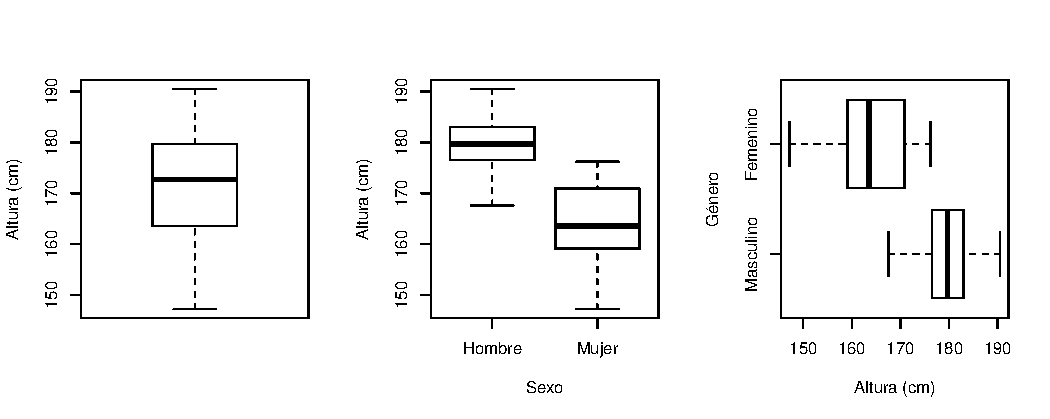
\includegraphics{02_graphs1v_files/figure-latex/boxplots-1.pdf}
\caption{\label{fig:boxplots}Boxplot para la variable altura.}
\end{figure}

En la Figura \ref{fig:boxplots} se presentan los boxplots obtenidos con
las instrucciones anteriores. El segundo y tercer boxplot son el mismo,
lo único que se modificó fueron los nombres o etiquetas a colocar debajo
de cada boxplot por medio del argumento \texttt{names} y la orientación.

\section{\texorpdfstring{Función
\texttt{hist}}{Función hist}}\label{funcion-hist}

La función \texttt{hist} sirve para crear el histograma
\index{histograma}\index{hist} para una variable cuantitativa. Como
argumentos esta función recibe un vector con los datos y opcionalmente
puede ingresarse como argumento el número de intervalos a ser graficados
o en su defecto el número de clases se determina con la fórmula de
Sturges.

Nota: los programas de computador usualmente construyen los histogramas
automáticamente, sin embargo, un buen programa debe permitirnos elegir
el número de intervalos del histograma. Si usted posee un programa que
no le permite hacer cambios, cambie de programa.

La estructura de la función \texttt{hist} con los argumentos más comunes
de uso se muestran a continuación.

\begin{itemize}
\tightlist
\item
  \texttt{x}: vector numérico de valores para construir el histograma.
\item
  \texttt{breaks}: puede ser un número entero que indica el número
  aproximado de clases o un vector cuyos elementos indican los límites
  de los intervalos.
\item
  \texttt{freq}: argumento lógico; si se especifica como \texttt{TRUE},
  el histograma presentará frecuencias absolutas o conteo de datos para
  cada intervalo; si se especifica como \texttt{FALSE} el histograma
  presentar las frecuencias relativas (en porcentaje). Por defecto, este
  argumento toma el valor de \texttt{TRUE} siempre y cuando los
  intervalos sean de igual ancho.
\item
  \texttt{include.lowest}: argumento lógico; si se especifica como
  \texttt{TRUE}, un \texttt{x{[}i{]}} igual a los equal a un valor
  \texttt{breaks\textquotesingle{}\textquotesingle{}\ se\ incluirá\ en\ la\ primera\ barra,\ si\ el\ argumento}right
  = TRUE'', o en la última en caso contrario.
\item
  \texttt{right}: argumento lógico; si es \texttt{TRUE}, los intervalos
  son abiertos a la izquierda y cerrados a la derecha \((a,b]\). Para la
  primera clase o intervalo si \texttt{include.lowest=TRUE} el valor más
  pequeño de los datos será incluido en éste. Si es \texttt{FALSE} los
  intervalos serán de la forma \([a,b)\) y el argumento
  \texttt{include.lowest=TRUE} tendrá el significado de incluir el ``más
  alto''.
\item
  \texttt{col}: para definir el color de las barras. Por defecto,
  \texttt{NULL} produce barras sin fondo.
\item
  \texttt{border}: para definir el color de los bordes de las barras.
\item
  \texttt{plot}: argumento lógico. Por defecto es \texttt{TRUE}, y el
  resultado es el gráfico del histograma; si se especifica como
  \texttt{FALSE} el resultado es una lista de conteos por cada
  intervalo.
\item
  \texttt{labels}: argumento lógico o carácter. Si se especifica como
  \texttt{TRUE} coloca etiquetas arriba de cada barra.
\item
  \texttt{...}: parámetros gráficos adicionales a \texttt{title} y
  \texttt{axis}.
\end{itemize}

\subsection*{Ejemplo}\label{ejemplo-2}
\addcontentsline{toc}{subsection}{Ejemplo}

Vamos a construir varios histogramas para los tiempos de 180 corredores
de la media maratón de CONAVI. A continuación se muestra la forma de
ingresar los 180 datos.

\begin{Shaded}
\begin{Highlighting}[]
\NormalTok{maraton <-}\StringTok{ }\KeywordTok{c}\NormalTok{(}
\DecValTok{10253}\NormalTok{, }\DecValTok{10302}\NormalTok{, }\DecValTok{10307}\NormalTok{, }\DecValTok{10309}\NormalTok{, }\DecValTok{10349}\NormalTok{, }\DecValTok{10353}\NormalTok{, }\DecValTok{10409}\NormalTok{, }\DecValTok{10442}\NormalTok{, }\DecValTok{10447}\NormalTok{, }\DecValTok{10452}\NormalTok{, }\DecValTok{10504}\NormalTok{, }\DecValTok{10517}\NormalTok{,}
\DecValTok{10530}\NormalTok{, }\DecValTok{10540}\NormalTok{, }\DecValTok{10549}\NormalTok{, }\DecValTok{10549}\NormalTok{, }\DecValTok{10606}\NormalTok{, }\DecValTok{10612}\NormalTok{, }\DecValTok{10646}\NormalTok{, }\DecValTok{10648}\NormalTok{, }\DecValTok{10655}\NormalTok{, }\DecValTok{10707}\NormalTok{, }\DecValTok{10726}\NormalTok{, }\DecValTok{10731}\NormalTok{,}
\DecValTok{10737}\NormalTok{, }\DecValTok{10743}\NormalTok{, }\DecValTok{10808}\NormalTok{, }\DecValTok{10833}\NormalTok{, }\DecValTok{10843}\NormalTok{, }\DecValTok{10920}\NormalTok{, }\DecValTok{10938}\NormalTok{, }\DecValTok{10949}\NormalTok{, }\DecValTok{10954}\NormalTok{, }\DecValTok{10956}\NormalTok{, }\DecValTok{10958}\NormalTok{, }\DecValTok{11004}\NormalTok{,}
\DecValTok{11009}\NormalTok{, }\DecValTok{11024}\NormalTok{, }\DecValTok{11037}\NormalTok{, }\DecValTok{11045}\NormalTok{, }\DecValTok{11046}\NormalTok{, }\DecValTok{11049}\NormalTok{, }\DecValTok{11104}\NormalTok{, }\DecValTok{11127}\NormalTok{, }\DecValTok{11205}\NormalTok{, }\DecValTok{11207}\NormalTok{, }\DecValTok{11215}\NormalTok{, }\DecValTok{11226}\NormalTok{,}
\DecValTok{11233}\NormalTok{, }\DecValTok{11239}\NormalTok{, }\DecValTok{11307}\NormalTok{, }\DecValTok{11330}\NormalTok{, }\DecValTok{11342}\NormalTok{, }\DecValTok{11351}\NormalTok{, }\DecValTok{11405}\NormalTok{, }\DecValTok{11413}\NormalTok{, }\DecValTok{11438}\NormalTok{, }\DecValTok{11453}\NormalTok{, }\DecValTok{11500}\NormalTok{, }\DecValTok{11501}\NormalTok{,}
\DecValTok{11502}\NormalTok{, }\DecValTok{11503}\NormalTok{, }\DecValTok{11527}\NormalTok{, }\DecValTok{11544}\NormalTok{, }\DecValTok{11549}\NormalTok{, }\DecValTok{11559}\NormalTok{, }\DecValTok{11612}\NormalTok{, }\DecValTok{11617}\NormalTok{, }\DecValTok{11635}\NormalTok{, }\DecValTok{11655}\NormalTok{, }\DecValTok{11731}\NormalTok{, }\DecValTok{11735}\NormalTok{,}
\DecValTok{11746}\NormalTok{, }\DecValTok{11800}\NormalTok{, }\DecValTok{11814}\NormalTok{, }\DecValTok{11828}\NormalTok{, }\DecValTok{11832}\NormalTok{, }\DecValTok{11841}\NormalTok{, }\DecValTok{11909}\NormalTok{, }\DecValTok{11926}\NormalTok{, }\DecValTok{11937}\NormalTok{, }\DecValTok{11940}\NormalTok{, }\DecValTok{11947}\NormalTok{, }\DecValTok{11952}\NormalTok{,}
\DecValTok{12005}\NormalTok{, }\DecValTok{12044}\NormalTok{, }\DecValTok{12113}\NormalTok{, }\DecValTok{12209}\NormalTok{, }\DecValTok{12230}\NormalTok{, }\DecValTok{12258}\NormalTok{, }\DecValTok{12309}\NormalTok{, }\DecValTok{12327}\NormalTok{, }\DecValTok{12341}\NormalTok{, }\DecValTok{12413}\NormalTok{, }\DecValTok{12433}\NormalTok{, }\DecValTok{12440}\NormalTok{,}
\DecValTok{12447}\NormalTok{, }\DecValTok{12530}\NormalTok{, }\DecValTok{12600}\NormalTok{, }\DecValTok{12617}\NormalTok{, }\DecValTok{12640}\NormalTok{, }\DecValTok{12700}\NormalTok{, }\DecValTok{12706}\NormalTok{, }\DecValTok{12727}\NormalTok{, }\DecValTok{12840}\NormalTok{, }\DecValTok{12851}\NormalTok{, }\DecValTok{12851}\NormalTok{, }\DecValTok{12937}\NormalTok{,}
\DecValTok{13019}\NormalTok{, }\DecValTok{13040}\NormalTok{, }\DecValTok{13110}\NormalTok{, }\DecValTok{13114}\NormalTok{, }\DecValTok{13122}\NormalTok{, }\DecValTok{13155}\NormalTok{, }\DecValTok{13205}\NormalTok{, }\DecValTok{13210}\NormalTok{, }\DecValTok{13220}\NormalTok{, }\DecValTok{13228}\NormalTok{, }\DecValTok{13307}\NormalTok{, }\DecValTok{13316}\NormalTok{,}
\DecValTok{13335}\NormalTok{, }\DecValTok{13420}\NormalTok{, }\DecValTok{13425}\NormalTok{, }\DecValTok{13435}\NormalTok{, }\DecValTok{13435}\NormalTok{, }\DecValTok{13448}\NormalTok{, }\DecValTok{13456}\NormalTok{, }\DecValTok{13536}\NormalTok{, }\DecValTok{13608}\NormalTok{, }\DecValTok{13612}\NormalTok{, }\DecValTok{13620}\NormalTok{, }\DecValTok{13646}\NormalTok{,}
\DecValTok{13705}\NormalTok{, }\DecValTok{13730}\NormalTok{, }\DecValTok{13730}\NormalTok{, }\DecValTok{13730}\NormalTok{, }\DecValTok{13747}\NormalTok{, }\DecValTok{13810}\NormalTok{, }\DecValTok{13850}\NormalTok{, }\DecValTok{13854}\NormalTok{, }\DecValTok{13901}\NormalTok{, }\DecValTok{13905}\NormalTok{, }\DecValTok{13907}\NormalTok{, }\DecValTok{13912}\NormalTok{,}
\DecValTok{13920}\NormalTok{, }\DecValTok{14000}\NormalTok{, }\DecValTok{14010}\NormalTok{, }\DecValTok{14025}\NormalTok{, }\DecValTok{14152}\NormalTok{, }\DecValTok{14208}\NormalTok{, }\DecValTok{14230}\NormalTok{, }\DecValTok{14344}\NormalTok{, }\DecValTok{14400}\NormalTok{, }\DecValTok{14455}\NormalTok{, }\DecValTok{14509}\NormalTok{, }\DecValTok{14552}\NormalTok{,}
\DecValTok{14652}\NormalTok{, }\DecValTok{15009}\NormalTok{, }\DecValTok{15026}\NormalTok{, }\DecValTok{15242}\NormalTok{, }\DecValTok{15406}\NormalTok{, }\DecValTok{15409}\NormalTok{, }\DecValTok{15528}\NormalTok{, }\DecValTok{15549}\NormalTok{, }\DecValTok{15644}\NormalTok{, }\DecValTok{15758}\NormalTok{, }\DecValTok{15837}\NormalTok{, }\DecValTok{15916}\NormalTok{,}
\DecValTok{15926}\NormalTok{, }\DecValTok{15948}\NormalTok{, }\DecValTok{20055}\NormalTok{, }\DecValTok{20416}\NormalTok{, }\DecValTok{20520}\NormalTok{, }\DecValTok{20600}\NormalTok{, }\DecValTok{20732}\NormalTok{, }\DecValTok{20748}\NormalTok{, }\DecValTok{20916}\NormalTok{, }\DecValTok{21149}\NormalTok{, }\DecValTok{21714}\NormalTok{, }\DecValTok{23256}\NormalTok{)}
\end{Highlighting}
\end{Shaded}

Los datos están codificados como por seis números en el formato hmmss,
donde h corresponde a las horas, mm a los minutos y ss a los segundos
necesarios para completar la maratón. Antes de construir los histogramas
es necesario convertir los tiempos anteriores almacenados en
\texttt{maraton} a horas, para esto se utiliza el siguiente código.

\begin{Shaded}
\begin{Highlighting}[]
\NormalTok{horas <-}\StringTok{ }\NormalTok{maraton %/%}\StringTok{ }\DecValTok{10000}
\NormalTok{min <-}\StringTok{ }\NormalTok{(maraton -}\StringTok{ }\NormalTok{horas *}\StringTok{ }\DecValTok{10000}\NormalTok{) %/%}\StringTok{ }\DecValTok{100}
\NormalTok{seg <-}\StringTok{ }\NormalTok{maraton -}\StringTok{ }\NormalTok{horas *}\StringTok{ }\DecValTok{10000} \NormalTok{-}\StringTok{ }\NormalTok{min *}\StringTok{ }\DecValTok{100}
\NormalTok{Tiempos <-}\StringTok{ }\NormalTok{horas +}\StringTok{ }\NormalTok{min /}\StringTok{ }\DecValTok{60} \NormalTok{+}\StringTok{ }\NormalTok{seg /}\StringTok{ }\DecValTok{3600}
\end{Highlighting}
\end{Shaded}

A continuación se muestra el código para construir cuatro histogramas
con 2, 4, 8 y 16 intervalos para los tiempos a partir de la variable
\texttt{Tiempos}.

\begin{Shaded}
\begin{Highlighting}[]
\KeywordTok{par}\NormalTok{(}\DataTypeTok{mfrow=}\KeywordTok{c}\NormalTok{(}\DecValTok{2}\NormalTok{,}\DecValTok{2}\NormalTok{))}

\KeywordTok{hist}\NormalTok{(}\DataTypeTok{x=}\NormalTok{Tiempos, }\DataTypeTok{breaks=}\DecValTok{2}\NormalTok{, }\DataTypeTok{main=}\StringTok{""}\NormalTok{, }\DataTypeTok{xlab=}\StringTok{"Tiempo (horas)"}\NormalTok{, }\DataTypeTok{ylab=}\StringTok{"Frecuencias"}\NormalTok{, }\DataTypeTok{las=}\DecValTok{1}\NormalTok{)}
\KeywordTok{mtext}\NormalTok{(}\StringTok{"(A)"}\NormalTok{, }\DataTypeTok{side=}\DecValTok{1}\NormalTok{, }\DataTypeTok{line=}\DecValTok{4}\NormalTok{, }\DataTypeTok{font=}\DecValTok{1}\NormalTok{)}
\KeywordTok{hist}\NormalTok{(}\DataTypeTok{x=}\NormalTok{Tiempos, }\DataTypeTok{breaks=}\DecValTok{4}\NormalTok{, }\DataTypeTok{main=}\StringTok{""}\NormalTok{, }\DataTypeTok{xlab=}\StringTok{"Tiempo (horas)"}\NormalTok{, }\DataTypeTok{ylab=}\StringTok{"Frecuencias"}\NormalTok{, }\DataTypeTok{las=}\DecValTok{1}\NormalTok{)}
\KeywordTok{mtext}\NormalTok{(}\StringTok{"(B)"}\NormalTok{, }\DataTypeTok{side=}\DecValTok{1}\NormalTok{, }\DataTypeTok{line=}\DecValTok{4}\NormalTok{, }\DataTypeTok{font=}\DecValTok{1}\NormalTok{)}
\KeywordTok{hist}\NormalTok{(}\DataTypeTok{x=}\NormalTok{Tiempos, }\DataTypeTok{breaks=}\DecValTok{8}\NormalTok{, }\DataTypeTok{main=}\StringTok{""}\NormalTok{, }\DataTypeTok{xlab=}\StringTok{"Tiempo (horas)"}\NormalTok{, }\DataTypeTok{ylab=}\StringTok{"Frecuencias"}\NormalTok{)}
\KeywordTok{mtext}\NormalTok{(}\StringTok{"(C)"}\NormalTok{, }\DataTypeTok{side=}\DecValTok{1}\NormalTok{, }\DataTypeTok{line=}\DecValTok{4}\NormalTok{, }\DataTypeTok{font=}\DecValTok{1}\NormalTok{)}
\KeywordTok{hist}\NormalTok{(}\DataTypeTok{x=}\NormalTok{Tiempos, }\DataTypeTok{breaks=}\DecValTok{16}\NormalTok{, }\DataTypeTok{main=}\StringTok{""}\NormalTok{, }\DataTypeTok{xlab=}\StringTok{"Tiempo (horas)"}\NormalTok{, }\DataTypeTok{ylab=}\StringTok{"Frecuencias"}\NormalTok{)}
\KeywordTok{mtext}\NormalTok{(}\StringTok{"(D)"}\NormalTok{, }\DataTypeTok{side=}\DecValTok{1}\NormalTok{, }\DataTypeTok{line=}\DecValTok{4}\NormalTok{, }\DataTypeTok{font=}\DecValTok{1}\NormalTok{)}
\end{Highlighting}
\end{Shaded}

\begin{figure}[htbp]
\centering
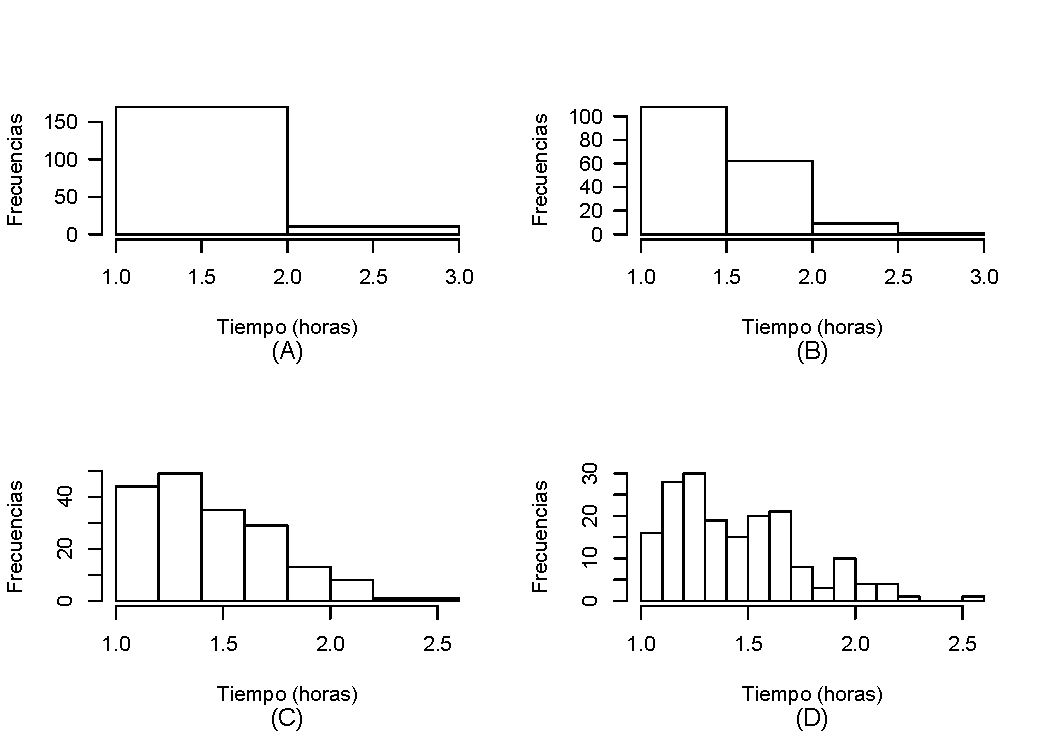
\includegraphics{02_graphs1v_files/figure-latex/hist1-1.pdf}
\caption{\label{fig:hist1}Histogramas para el tiempo en la media maratón de
CONAVI. A: histograma con dos intervalos, B: histograma con cuatro
intervalos, C: histograma con seis intervalos, C: histograma con 18
intervalos.}
\end{figure}

En la Figura \ref{fig:hist1} se presentan los cuatro histogramas. El
histograma C, con 8 barras, muestra más claramente la asimetría (este es
el que la mayoría de los programas produce por defecto, ya que la regla
de Sturges para este conjunto de datos aproxima a 8 barras). Si
consideramos más barras por ejemplo 16, como tenemos en D, se refina más
la información y empezamos a notar multimodalidad. En el código anterior
se incluyó \texttt{las\ =\ 1} para conseguir que los número del eje Y
queden escritos de forma horizontal, ver A y B en Figura
\ref{fig:hist1}.

A continuación vamos a construir cuatro histogramas: el primero con dos
intervalos intervalos y puntos de corte dados por el mínimo, la mediana
y el máximo; el segundo con tres intervalos y puntos de corte dados por
el mínimo, cuartiles 1, 2, 3 y máximo; el cuarto con diez intervalos y
puntos de corte dados por los deciles; y el último con veinte intervalos
y puntos de corte dados por cuantiles 5, 10, \(\ldots\), 95. En el
código mostrado a continuación se presenta la creación de los puntos de
corte y los cuatro histogramas.

\begin{Shaded}
\begin{Highlighting}[]
\NormalTok{puntos1 <-}\StringTok{ }\KeywordTok{c}\NormalTok{(}\KeywordTok{quantile}\NormalTok{(Tiempos, }\DataTypeTok{probs=}\KeywordTok{c}\NormalTok{(}\DecValTok{0}\NormalTok{, }\FloatTok{0.5}\NormalTok{, }\DecValTok{1}\NormalTok{)))}
\NormalTok{puntos2 <-}\StringTok{ }\KeywordTok{c}\NormalTok{(}\KeywordTok{quantile}\NormalTok{(Tiempos, }\DataTypeTok{probs=}\KeywordTok{c}\NormalTok{(}\DecValTok{0}\NormalTok{, }\FloatTok{0.25}\NormalTok{, }\FloatTok{0.5}\NormalTok{, }\FloatTok{0.75}\NormalTok{, }\DecValTok{1}\NormalTok{)))}
\NormalTok{puntos3 <-}\StringTok{ }\KeywordTok{c}\NormalTok{(}\KeywordTok{quantile}\NormalTok{(Tiempos, }\DataTypeTok{probs=}\KeywordTok{seq}\NormalTok{(}\DecValTok{0}\NormalTok{, }\DecValTok{1}\NormalTok{, }\DataTypeTok{by=}\FloatTok{0.1}\NormalTok{)))}
\NormalTok{puntos4 <-}\StringTok{ }\KeywordTok{c}\NormalTok{(}\KeywordTok{quantile}\NormalTok{(Tiempos, }\DataTypeTok{probs=}\KeywordTok{seq}\NormalTok{(}\DecValTok{0}\NormalTok{, }\DecValTok{1}\NormalTok{, }\DataTypeTok{by=}\FloatTok{0.05}\NormalTok{)))}

\KeywordTok{par}\NormalTok{(}\DataTypeTok{mfrow=}\KeywordTok{c}\NormalTok{(}\DecValTok{2}\NormalTok{, }\DecValTok{2}\NormalTok{))}
\KeywordTok{hist}\NormalTok{(Tiempos, }\DataTypeTok{breaks=}\NormalTok{puntos1, }\DataTypeTok{freq=}\OtherTok{FALSE}\NormalTok{, }\DataTypeTok{ylim=}\KeywordTok{c}\NormalTok{(}\DecValTok{0}\NormalTok{,}\DecValTok{2}\NormalTok{), }\DataTypeTok{labels=}\OtherTok{TRUE}\NormalTok{,}
     \DataTypeTok{main=}\StringTok{""}\NormalTok{, }\DataTypeTok{ylab=}\StringTok{"Densidad"}\NormalTok{)}
\KeywordTok{mtext}\NormalTok{(}\StringTok{"(A)"}\NormalTok{, }\DataTypeTok{side=}\DecValTok{1}\NormalTok{, }\DataTypeTok{line=}\DecValTok{4}\NormalTok{, }\DataTypeTok{font=}\DecValTok{1}\NormalTok{)}
\KeywordTok{hist}\NormalTok{(Tiempos, }\DataTypeTok{breaks=}\NormalTok{puntos2, }\DataTypeTok{freq=}\OtherTok{FALSE}\NormalTok{, }\DataTypeTok{ylim=}\KeywordTok{c}\NormalTok{(}\DecValTok{0}\NormalTok{,}\DecValTok{2}\NormalTok{), }\DataTypeTok{labels=}\OtherTok{TRUE}\NormalTok{,}
     \DataTypeTok{main=}\StringTok{""}\NormalTok{, }\DataTypeTok{ylab=}\StringTok{"Densidad"}\NormalTok{)}
\KeywordTok{mtext}\NormalTok{(}\StringTok{"(B)"}\NormalTok{, }\DataTypeTok{side=}\DecValTok{1}\NormalTok{, }\DataTypeTok{line=}\DecValTok{4}\NormalTok{, }\DataTypeTok{font=}\DecValTok{1}\NormalTok{)}
\KeywordTok{hist}\NormalTok{(Tiempos, }\DataTypeTok{breaks=}\NormalTok{puntos3, }\DataTypeTok{freq=}\OtherTok{FALSE}\NormalTok{, }\DataTypeTok{ylim=}\KeywordTok{c}\NormalTok{(}\DecValTok{0}\NormalTok{,}\DecValTok{2}\NormalTok{),}
     \DataTypeTok{main=}\StringTok{""}\NormalTok{, }\DataTypeTok{ylab=}\StringTok{"Densidad"}\NormalTok{)}
\KeywordTok{mtext}\NormalTok{(}\StringTok{"(C)"}\NormalTok{, }\DataTypeTok{side=}\DecValTok{1}\NormalTok{, }\DataTypeTok{line=}\DecValTok{4}\NormalTok{, }\DataTypeTok{font=}\DecValTok{1}\NormalTok{)}
\KeywordTok{hist}\NormalTok{(Tiempos, }\DataTypeTok{breaks=}\NormalTok{puntos4, }\DataTypeTok{freq=}\OtherTok{FALSE}\NormalTok{, }\DataTypeTok{ylim=}\KeywordTok{c}\NormalTok{(}\DecValTok{0}\NormalTok{,}\DecValTok{2}\NormalTok{),}
     \DataTypeTok{main=}\StringTok{""}\NormalTok{, }\DataTypeTok{ylab=}\StringTok{"Densidad"}\NormalTok{)}
\KeywordTok{mtext}\NormalTok{(}\StringTok{"(D)"}\NormalTok{, }\DataTypeTok{side=}\DecValTok{1}\NormalTok{, }\DataTypeTok{line=}\DecValTok{4}\NormalTok{, }\DataTypeTok{font=}\DecValTok{1}\NormalTok{)}
\end{Highlighting}
\end{Shaded}

\begin{figure}[htbp]
\centering
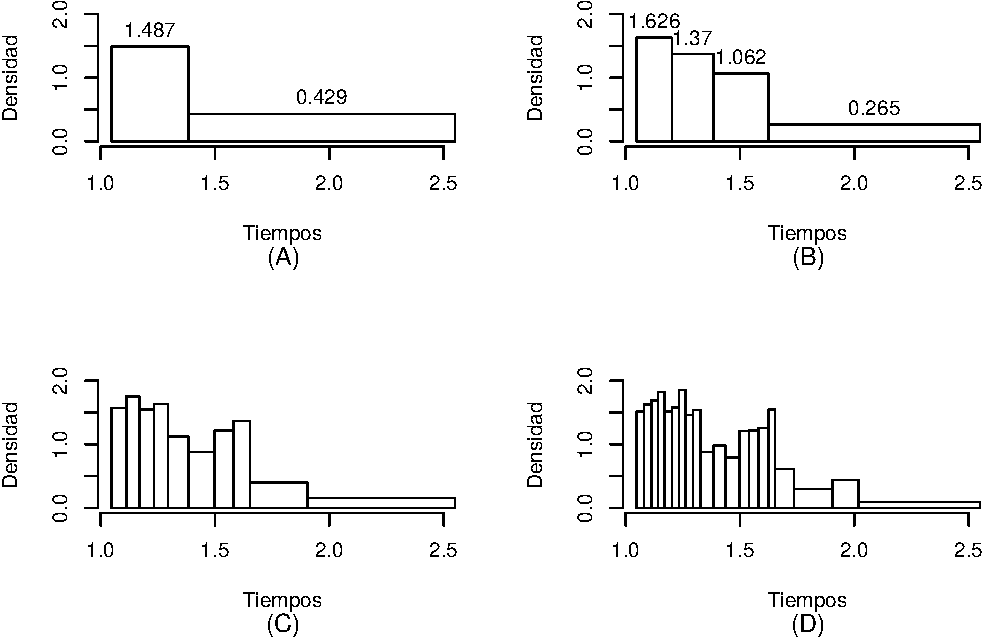
\includegraphics{02_graphs1v_files/figure-latex/hist2-1.pdf}
\caption{\label{fig:hist2}Histogramas para el tiempo en la media maratón de
CONAVI. A: histograma con dos intervalos, B: histograma con cuatro
intervalos, C: histograma con diez intervalos, C: histograma con veinte
intervalos.}
\end{figure}

Nota: En estos histogramas, las alturas corresponden a las intensidades
(frec. relativa/long. intervalo). Por tanto, el área de cada rectángulo
da cuenta de las frecuencias relativas. Para el caso (A) ambos
intervalos tienen igual área y cada uno contiene 50\% de los datos. esto
puede verificarse así:

\begin{verbatim}
Intensidad primera clase = 1.4869888 = 0.5 / (1.384306 - 1.048056)
Intensidad segunda clase = 0.4293381 = 0.5 / (2.548889 - 1.384306)
\end{verbatim}

\section{\texorpdfstring{Función \texttt{qqnorm} y \texttt{qqplot}
\index{qqnorm}
\index{qqplot}}{Función qqnorm y qqplot  }}\label{funcion-qqnorm-y-qqplot}

Los gráficos cuantil cuantil (quantile-quantile plot) son una ayuda para
explorar si un conjunto de datos o muestra proviene de una población con
cierta distribución.

La función \texttt{qqnorm} sirve para explorar la normalidad de una
muestra mientras que la función \texttt{qqplot} es de propósito más
general, sirve para crear el gráfico cuantil cuantil para cualquier
distribución.

La estructura de las funciones con los argumentos más comunes de uso se
muestran a continuación.

\begin{Shaded}
\begin{Highlighting}[]
\KeywordTok{qqnorm}\NormalTok{(y, ...)}
\KeywordTok{qqplot}\NormalTok{(y, x, ...)}
\end{Highlighting}
\end{Shaded}

La función \texttt{qqnorm} sólo necesita que se le ingrese el vector con
la muestra por medio del parámetro \texttt{y}, la función
\texttt{qqplot} necesita de la muestra en el parámetro \texttt{y} y que
se ingrese en el parámetro \texttt{x} los cuantiles de la población
candidata.

Existe otra función útil y es \texttt{qqline}, esta función sirve para
agregar una línea de referencia al gráfico cuantil cuantil obtenido con
\texttt{qqnorm}.

\subsection*{Ejemplo}\label{ejemplo-3}
\addcontentsline{toc}{subsection}{Ejemplo}

Simular 30 observaciones de una distribución \(N(\mu=10, \sigma=4)\) y
construir el gráfico cuantil cuantil.

El código para simular la muestra y crear el gráfico cuantil cuantil se
muestra a continuación.

\begin{Shaded}
\begin{Highlighting}[]
\NormalTok{muestra <-}\StringTok{ }\KeywordTok{rnorm}\NormalTok{(}\DataTypeTok{n=}\DecValTok{30}\NormalTok{, }\DataTypeTok{mean=}\DecValTok{10}\NormalTok{, }\DataTypeTok{sd=}\DecValTok{4}\NormalTok{)}

\KeywordTok{par}\NormalTok{(}\DataTypeTok{mfrow=}\KeywordTok{c}\NormalTok{(}\DecValTok{1}\NormalTok{, }\DecValTok{2}\NormalTok{))}
\KeywordTok{qqnorm}\NormalTok{(}\DataTypeTok{y=}\NormalTok{muestra)}
\KeywordTok{qqline}\NormalTok{(}\DataTypeTok{y=}\NormalTok{muestra)}

\KeywordTok{qqnorm}\NormalTok{(}\DataTypeTok{y=}\NormalTok{muestra, }\DataTypeTok{main=}\StringTok{''}\NormalTok{, }\DataTypeTok{ylab=}\StringTok{'Cuantiles muestrales'}\NormalTok{,}
       \DataTypeTok{xlab=}\StringTok{'Cuantiles teóricos'}\NormalTok{, }\DataTypeTok{las=}\DecValTok{1}\NormalTok{)}
\KeywordTok{qqline}\NormalTok{(}\DataTypeTok{y=}\NormalTok{muestra, }\DataTypeTok{col=}\StringTok{'blue'}\NormalTok{, }\DataTypeTok{lwd=}\DecValTok{2}\NormalTok{)}
\end{Highlighting}
\end{Shaded}

\begin{figure}[htbp]
\centering
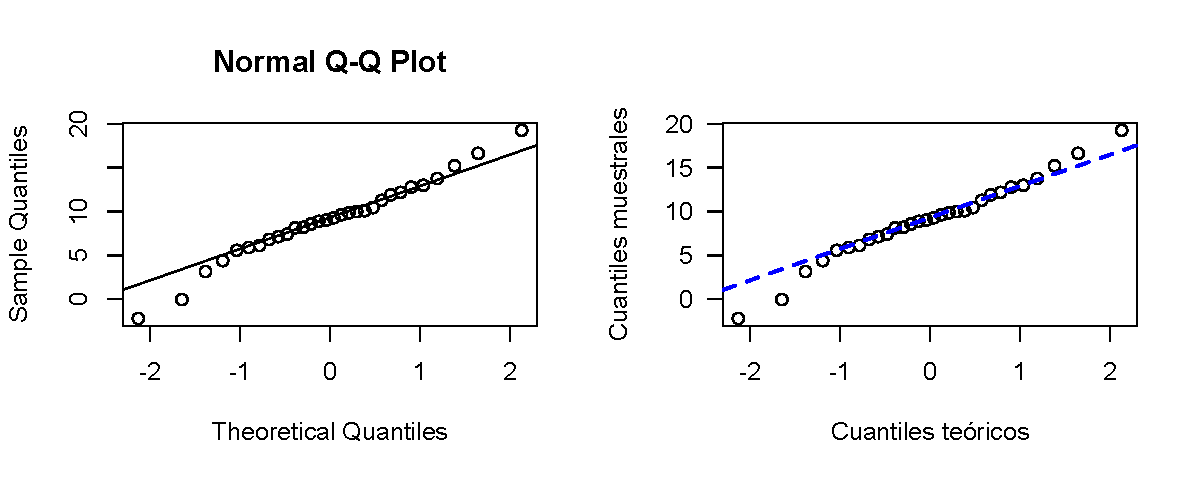
\includegraphics{02_graphs1v_files/figure-latex/qqplot1-1.pdf}
\caption{\label{fig:qqplot1}Gráfico cuantil cuantil para una muestra
generada de una población normal.}
\end{figure}

En la izquierda de la Figura \ref{fig:qqplot1} está el gráfico cuantil
cuantil sin editar, en la derecha se encuentra el gráfico luego de
modificar los nombres de los ejes, grosor y color de la línea de
referencia.

\subsection*{Ejemplo}\label{ejemplo-4}
\addcontentsline{toc}{subsection}{Ejemplo}

Simular 100 observaciones de una distribución \(Weibull(1,1)\) y
construir dos gráficos cuantil cuantil, el primero tomando como
referencia los cuantiles de una \(N(0,1)\) y el segundo tomando los
cuantiles de la \(Weibull(1,1)\).

El código para simular la muestra y crear los gráficos cuantil cuantil
se muestra a continuación.

\begin{Shaded}
\begin{Highlighting}[]
\NormalTok{n <-}\StringTok{ }\DecValTok{100}
\NormalTok{muestra <-}\StringTok{ }\KeywordTok{rweibull}\NormalTok{(}\DataTypeTok{n=}\NormalTok{n, }\DataTypeTok{shape=}\DecValTok{1}\NormalTok{, }\DataTypeTok{scale=}\DecValTok{1}\NormalTok{)}

\KeywordTok{par}\NormalTok{(}\DataTypeTok{mfrow=}\KeywordTok{c}\NormalTok{(}\DecValTok{1}\NormalTok{, }\DecValTok{2}\NormalTok{))}
\KeywordTok{qqplot}\NormalTok{(}\DataTypeTok{y=}\NormalTok{muestra, }\DataTypeTok{x=}\KeywordTok{qnorm}\NormalTok{(}\KeywordTok{ppoints}\NormalTok{(n)))}
\KeywordTok{qqplot}\NormalTok{(}\DataTypeTok{y=}\NormalTok{muestra, }\DataTypeTok{x=}\KeywordTok{qweibull}\NormalTok{(}\KeywordTok{ppoints}\NormalTok{(n), }\DataTypeTok{shape=}\DecValTok{1}\NormalTok{, }\DataTypeTok{scale=}\DecValTok{1}\NormalTok{))}
\end{Highlighting}
\end{Shaded}

\begin{figure}[htbp]
\centering
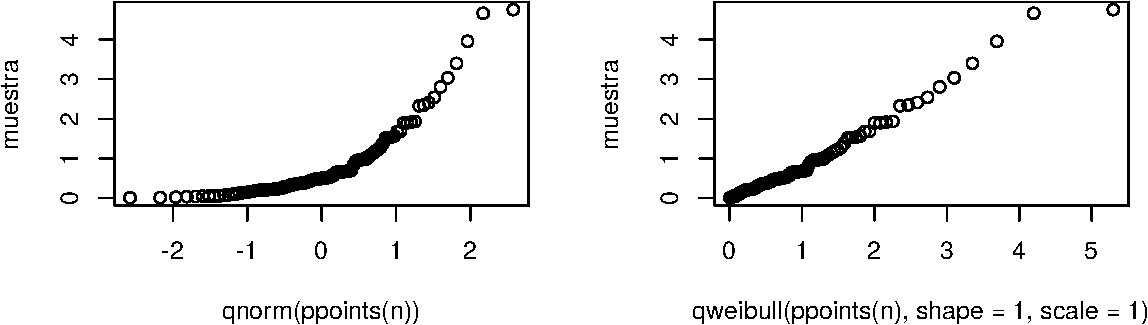
\includegraphics{02_graphs1v_files/figure-latex/qqplot2-1.pdf}
\caption{\label{fig:qqplot2}Gráfico cuantil cuantil para una muestra
generada de una población Weibull.}
\end{figure}

En la Figura \ref{fig:qqplot2} están los gráficos cuantil cuantil
solicitados. Del pánel izquierdo de la figura vemos que los puntos NO
están alineados, esto indica que la muestra no proviene de la
distribución \(N(0, 1)\), esto es un resultado esperado ya que sabíamos
que la muestra no fue generada de una normal. En el pánel derecho de la
misma figura vemos que los puntos SI están alineados, esto indica que la
muestra generada puede provenir de una población \(Weibull(1, 1)\). Los
nombres de los ejes en la Figura \ref{fig:qqplot2} pueden ser editados
para presentar una figura con mejor apariencia.

\bibliography{packages,book}

\printindex


\end{document}
